\documentclass[12pt]{article}

\usepackage{amsmath}
\usepackage{amssymb}
\usepackage{physics}
\usepackage{enumitem}
\usepackage{tikz}
\usetikzlibrary{arrows.meta,calc,angles,quotes,decorations.pathmorphing}
\usepackage{geometry}
\geometry{margin=1in}

\begin{document}

\begin{center}
{\Large \textbf{SET 18 (Ultra-Hard JEE Advanced – Fully Stabilized Final Paper)}}
\end{center}

\begin{enumerate}[leftmargin=*]

%====================================================
\item A conducting rod of mass $m$ and length $l$ is free to slide without friction on two parallel conducting rails which are rigidly fixed on a smooth incline making an angle $\theta$ with the horizontal. The rod remains perpendicular to the rails at all times. Its upper end is connected to a light spring of force constant $k$ whose other end is rigidly fixed along the incline. The lower ends of the rails are connected through a resistor $R$, forming a closed circuit. A uniform magnetic field $B$ is applied perpendicular to the plane of the rails (into the page). If the rod is slightly displaced from its equilibrium position and released, it executes damped oscillations due to electromagnetic induction. For small oscillations, the condition for underdamped motion is

\begin{center}
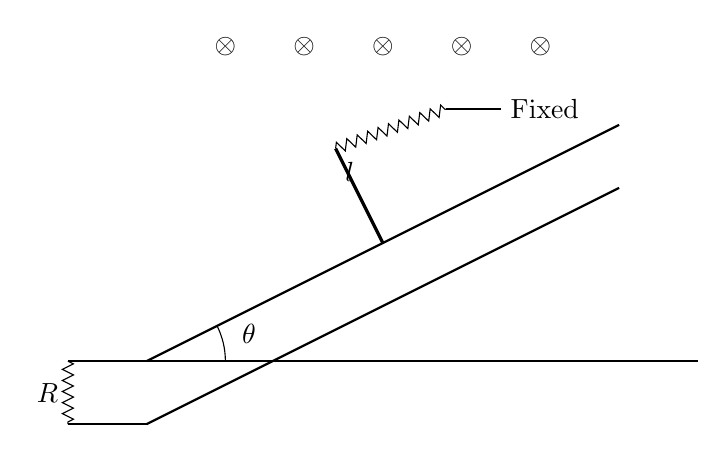
\begin{tikzpicture}[scale=1]

% Ground
\draw[thick] (-0.5,0) -- (7,0);

% Upper rail
\draw[thick] (0,0) -- (6,3);

% Lower rail
\draw[thick] (0,-0.8) -- (6,2.2);

% Angle theta
\draw (1,0) arc (0:26.565:1);
\node at (1.3,0.35) {$\theta$};

% Rod perpendicular to incline
\draw[very thick] (3,1.5) -- (2.4,2.7);
\node[right] at (2.4,2.4) {$l$};

% Spring
\draw[decorate, decoration={zigzag, segment length=4pt, amplitude=2pt}]
(2.4,2.7) -- (3.8,3.2);
\draw[thick] (3.8,3.2) -- (4.5,3.2);
\node[right] at (4.5,3.2) {Fixed};

% Resistor
\draw[thick] (0,0) -- (-1,0);
\draw[decorate, decoration={zigzag, segment length=4pt, amplitude=2pt}]
(-1,0) -- (-1,-0.8);
\draw[thick] (-1,-0.8) -- (0,-0.8);
\node[left] at (-1,-0.4) {$R$};

% Magnetic field
\foreach \x in {1,2,3,4,5}
{
\node at (\x,4) {$\otimes$};
}

\end{tikzpicture}
\end{center}

\begin{enumerate}
\item $\dfrac{B^2 l^2}{R} < 2\sqrt{km}$
\item $\dfrac{B^2 l^2}{R} > 2\sqrt{km}$
\item $\dfrac{B l}{R} < \sqrt{km}$
\item $\dfrac{B^2 l}{R} < \sqrt{km}$
\end{enumerate}

%====================================================
\item A particle of mass $m$ moves under a central force derived from the potential 
$V(r)= -\dfrac{k}{r} + \dfrac{\alpha}{r^2} + \beta r^2$, 
where $k>0$, $\alpha>0$, and $\beta>0$ are constants. For a circular orbit of radius $r_0$, stability requires that the second derivative of the effective potential with respect to $r$ evaluated at $r=r_0$ be positive. Eliminating the angular momentum using the equilibrium condition for circular motion, the inequality for stable orbit becomes

\begin{enumerate}
\item $\beta r_0^4 > \alpha$
\item $3\beta r_0^4 > \alpha$
\item $\beta r_0^4 < \alpha$
\item $2\beta r_0^4 > \alpha$
\end{enumerate}

%====================================================
\item A dielectric slab of mass $m$ and dielectric constant $K$ partially fills a horizontal parallel plate capacitor of area $A$ and separation $d$. The capacitor is connected to a battery maintaining constant voltage $V$. The slab is attached to a spring of force constant $k$ fixed to a rigid support. Neglecting edge effects and assuming small oscillations about equilibrium, the angular frequency of oscillation is

\begin{enumerate}
\item $\sqrt{\dfrac{k + \dfrac{\epsilon_0 A V^2 (K-1)}{d^2}}{m}}$
\item $\sqrt{\dfrac{k}{m}}$
\item $\sqrt{\dfrac{\epsilon_0 A V^2 (K-1)}{m d^2}}$
\item $\sqrt{\dfrac{k - \dfrac{\epsilon_0 A V^2 (K-1)}{d^2}}{m}}$
\end{enumerate}

%====================================================
\item A rigid rectangular conducting coil of area $A$, resistance $R$, and moment of inertia $I$ is free to rotate about a vertical axis passing through its centre. The coil is placed in a uniform magnetic field $B$ directed into the page. When displaced slightly and released, induced currents produce a damping torque proportional to angular velocity for small motion. The effective damping coefficient is

\begin{enumerate}
\item $\dfrac{B^2 A^2}{R}$
\item $\dfrac{BA}{R}$
\item $\dfrac{B^2 A}{R}$
\item $\dfrac{B A^2}{R}$
\end{enumerate}

%====================================================
\item Consider an isothermal column of an ideal gas in thermal equilibrium in a uniform gravitational field $g$. The gas consists of molecules of mass $m$, and temperature is maintained constant at $T$ throughout the column. Using hydrostatic equilibrium and the ideal gas equation of state, the scale height governing exponential pressure variation is

\begin{enumerate}
\item $\dfrac{kT}{mg}$
\item $\dfrac{mg}{kT}$
\item $\dfrac{RT}{g}$
\item $\dfrac{g}{RT}$
\end{enumerate}

%====================================================
\item The root-mean-square speed of molecules in an ideal gas is $v_{\text{rms}}=\sqrt{\dfrac{3kT}{m}}$. If temperature increases by a small amount $\Delta T$ with $\Delta T \ll T$, the fractional change in $v_{\text{rms}}$ to first order is

\begin{enumerate}
\item $\dfrac{1}{2}\dfrac{\Delta T}{T}$
\item $\dfrac{\Delta T}{T}$
\item $\dfrac{3}{2}\dfrac{\Delta T}{T}$
\item $\dfrac{\Delta T}{2T^2}$
\end{enumerate}

%====================================================
\item A series RLC circuit having resistance $R$, inductance $L$, and capacitance $C$ is driven by an AC source of variable frequency. The circuit exhibits resonance at angular frequency $\omega_0$. If the quality factor of the circuit is $Q$, the bandwidth between half-power frequencies is

\begin{enumerate}
\item $\dfrac{\omega_0}{Q}$
\item $\omega_0 Q$
\item $\dfrac{\omega_0}{2Q}$
\item $\dfrac{2\omega_0}{Q}$
\end{enumerate}

%====================================================
\item In Young’s double-slit experiment, monochromatic light of wavelength $\lambda$ produces an interference pattern on a screen at distance $D$ from the slits separated by distance $d$. If the slit separation is doubled while keeping all other parameters unchanged, the fringe width on the screen becomes

\begin{enumerate}
\item Half of its original value
\item Twice its original value
\item Unchanged
\item Four times its original value
\end{enumerate}

%====================================================
\item A thin film of refractive index $\mu$ is illuminated normally by light of wavelength $\lambda$ in air. Considering phase reversal at the first interface only, the minimum thickness for constructive interference in reflected light is

\begin{enumerate}
\item $\dfrac{\lambda}{4\mu}$
\item $\dfrac{\lambda}{2\mu}$
\item $\dfrac{\lambda}{\mu}$
\item $\dfrac{3\lambda}{4\mu}$
\end{enumerate}

%====================================================
\item Expanding relativistic momentum $p=\gamma mv$ in powers of $v/c$, the first correction term beyond classical momentum $mv$ is proportional to

\begin{enumerate}
\item $\dfrac{mv^3}{c^2}$
\item $\dfrac{mv^2}{c^2}$
\item $\dfrac{mv^4}{c^2}$
\item $\dfrac{mv^3}{c^4}$
\end{enumerate}

%====================================================
\item In a radioactive decay chain $A \to B \to C$, where decay constants are $\lambda_1$ and $\lambda_2$ respectively, and initially only $A$ is present, the time at which the number of nuclei of intermediate product $B$ is maximum is

\begin{enumerate}
\item $\dfrac{1}{\lambda_2-\lambda_1}\ln\dfrac{\lambda_2}{\lambda_1}$
\item $\dfrac{1}{\lambda_1}\ln\dfrac{\lambda_2}{\lambda_1}$
\item $\dfrac{1}{\lambda_2}\ln\dfrac{\lambda_1}{\lambda_2}$
\item $\dfrac{1}{\lambda_1-\lambda_2}\ln\dfrac{\lambda_1}{\lambda_2}$
\end{enumerate}

%====================================================
\item An ideal Zener diode is used for voltage regulation. If the input voltage increases slightly while the load resistance remains constant and the diode operates in breakdown region, the fractional change in output voltage is

\begin{enumerate}
\item Zero
\item $\dfrac{\Delta V}{V_Z}$
\item $\dfrac{\Delta V}{V}$
\item $\dfrac{R_L}{R}\dfrac{\Delta V}{V}$
\end{enumerate}

%====================================================
\item In single-slit diffraction using light of wavelength $\lambda$, the angular width of the central maximum is inversely proportional to the slit width. If the slit width is reduced to half while keeping wavelength fixed, the angular width of the central maximum becomes

\begin{enumerate}
\item Twice the original value
\item Half the original value
\item Unchanged
\item One-fourth the original value
\end{enumerate}

%====================================================
\item In the photoelectric effect, light of frequency greater than threshold frequency is incident on a metal surface. The threshold frequency depends on

\begin{enumerate}
\item The intensity of incident light
\item The work function of the metal
\item The applied stopping potential
\item The distance between source and metal
\end{enumerate}

%====================================================
\item The root-mean-square speed of molecules in an ideal gas is proportional to the square root of absolute temperature. If temperature is increased fourfold while molecular mass remains unchanged, the new RMS speed becomes

\begin{enumerate}
\item Twice the original value
\item Four times the original value
\item Half the original value
\item Unchanged
\end{enumerate}

\end{enumerate}

\end{document}
